\documentclass{article}
\usepackage{graphicx} % Required for inserting images
\usepackage{float}
\usepackage[T1]{fontenc}
\usepackage{amsmath}
\usepackage[margin=1in]{geometry}
\usepackage{booktabs}
\usepackage{tabularx}
\usepackage[hidelinks]{hyperref}

\title{A small crash call beside the stress-sized put book}
\author{Experiment report \textperiodcentered{} L/S Gamma Desk, QUANTT}
\date{2026-11-02}

\begin{document}

\maketitle

\textbf{Question:} On the 35\% stress-sized \texttt{hedged} put book, does also buying at-the-money calls with 0.5\% of capital whenever the VIX curve is inverted (VIX/\allowbreak{}VIX3M at least 1.1 at the prior close) make the maximum drawdown and the 5\% expected shortfall less severe, at a cost of no more than \$10,000 of net P\&L?

\textbf{Method:}

\begin{itemize}

\item \textbf{Pre-registered backtest:} the hypothesis card was committed before any run (commit 3568520). The research switches were committed before it (a2d5334).

\item \textbf{Data:} the live paper rules (\texttt{configs/\allowbreak{}paper.\allowbreak{}toml}) are replayed on R2 replay snapshots v1 (config\_hash b040760187f0) over the development window 2014-06-02 to 2024-12-31. The hold-out (2025-01-01 to 2026-07-10) was not used.

\item \textbf{Book (every variant and the reference):} the \texttt{hedged} book of \texttt{2026-\allowbreak{}10-\allowbreak{}22-\allowbreak{}stress-\allowbreak{}sized-\allowbreak{}puts}.

\begin{itemize}

\item An always-on short 25-delta put, with the signal ignored and the flat exit off.

\item Sized at entry so that a one-day 20\% SPY drop, with IV at max(60\%, the put's IV), costs at most 35\% of \$250k (\$87,500).

\item A 10-share daily hedge, the 1x-credit stop, the 50\% profit-take, the 7-DTE time exit and the 1-day cool-off.

\end{itemize}

\item \textbf{The crash call} (new research switches \texttt{crash\_\allowbreak{}gate}, \texttt{crash\_\allowbreak{}dte}, \texttt{crash\_\allowbreak{}days}, \texttt{crash\_\allowbreak{}premium}):

\begin{itemize}

\item At the 10:15 decision, if VIX/\allowbreak{}VIX3M at the prior close is at or above the gate and no crash call is open, the book buys at-the-money calls with 0.5\% of capital (\$1,250).

\item The call is held 5 trading days, with no stop, profit-take or flat exit; if the gate is still on when it closes, a new one is bought at the same step.

\item It sits beside the put (it does not use the put's slot) and is not counted in the put's stress test. Its delta joins the book's daily 10-share hedge.

\end{itemize}

\item \textbf{Variants:}

\begin{itemize}

\item \texttt{crash11} (primary): gate 1.1, expiry 8-14 days (target 10).

\item \texttt{crash10} (sensitivity): gate 1.0.

\item \texttt{crash11\_\allowbreak{}30d} (sensitivity): gate 1.1, expiry 21-45 days (target 30, the desk's usual long call).

\end{itemize}

\item \textbf{Comparison:} the registered \texttt{2026-\allowbreak{}10-\allowbreak{}22-\allowbreak{}stress-\allowbreak{}sized-\allowbreak{}puts/\allowbreak{}hedged} runs at the same spread multiple, reused and not rerun. With the switches off, the engine reproduces their equity exactly.

\item \textbf{Runs and costs:} every variant was run at 1x and 2x spreads. Costs are \$0.65 per contract and \$0.005 per share, with a \$1 minimum per order. Decisions and hedges run at 10:15 ET; decisions read a 15-minute-old chain, and fills price on trades in the 15 minutes after. Spot comes from put-call parity on the 30-minute snapshot grid (10:15-15:45).

\end{itemize}

\section{Result vs the pass bar}

Every check had to hold at 1x and 2x. P\&L is net of costs in USD for the whole book. ES is the mean of the worst 5\% of daily P\&L.

\begin{center}\small
\begin{tabularx}{\linewidth}{>{\raggedright\arraybackslash}X l >{\raggedright\arraybackslash}X l >{\raggedright\arraybackslash}X l}
\toprule
\textbf{Check (\texttt{crash11} vs \texttt{hedged})} & \textbf{1x value} & \textbf{1x bar} & \textbf{2x value} & \textbf{2x bar} & \textbf{Result} \\
\midrule
Max drawdown less severe & \$70,998 & < \$70,362 & \$76,514 & < \$75,488 & fail \\
ES 5\% less severe & \ensuremath{-}\$2,998 & better than \ensuremath{-}\$3,016 & \ensuremath{-}\$3,077 & better than \ensuremath{-}\$3,094 & pass \\
Net P\&L not below hedged \ensuremath{-} \$10,000 & \$119,806 & \ensuremath{\geq} \$111,482 & \$98,891 & \ensuremath{\geq} \$91,172 & pass \\
Event floor: crash calls opened \ensuremath{\geq} 10 & 14 & \ensuremath{\geq} 10 &  &  & met \\
\bottomrule
\end{tabularx}
\end{center}

\textbf{Verdict: failed.}

\begin{itemize}

\item The crash call made the drawdown slightly worse: by \$636 at 1x and \$1,026 at 2x.

\item It barely moved anything else. ES improved by about \$18 a day, and net P\&L fell by \$1,675 at 1x and \$2,281 at 2x.

\item At this size, the call is too small to change the put book's risk either way.

\end{itemize}

\subsection{Full-window numbers (not part of the bar)}

\textbf{1x spreads}

\begin{center}\small
\begin{tabularx}{\linewidth}{>{\raggedright\arraybackslash}X l l l >{\raggedright\arraybackslash}X}
\toprule
\textbf{} & \textbf{\texttt{hedged}} & \textbf{\texttt{crash11}} & \textbf{\texttt{crash10}} & \textbf{\texttt{crash11\_\allowbreak{}30d}} \\
\midrule
Net P\&L & \$121,482 & \$119,806 & \$114,556 & \$122,191 \\
Sharpe & 0.52 & 0.51 & 0.49 & 0.52 \\
Max drawdown & \$70,362 & \$70,998 & \$73,546 & \$69,497 \\
ES 5\% (daily) & \ensuremath{-}\$3,016 & \ensuremath{-}\$2,998 & \ensuremath{-}\$2,957 & \ensuremath{-}\$2,998 \\
Round trips (puts + calls) & 182 & 196 & 241 & 194 \\
Crash calls opened & 0 & 14 & 59 & 12 \\
Option commissions & \$5,955 & \$5,995 & \$6,156 & \$5,982 \\
Hedge commissions & \$2,868 & \$2,866 & \$2,865 & \$2,867 \\
\bottomrule
\end{tabularx}
\end{center}

\textbf{2x spreads}

\begin{center}\small
\begin{tabularx}{\linewidth}{>{\raggedright\arraybackslash}X l l l >{\raggedright\arraybackslash}X}
\toprule
\textbf{} & \textbf{\texttt{hedged}} & \textbf{\texttt{crash11}} & \textbf{\texttt{crash10}} & \textbf{\texttt{crash11\_\allowbreak{}30d}} \\
\midrule
Net P\&L & \$101,172 & \$98,891 & \$94,124 & \$101,753 \\
Sharpe & 0.43 & 0.42 & 0.40 & 0.43 \\
Max drawdown & \$75,488 & \$76,514 & \$80,278 & \$74,732 \\
ES 5\% (daily) & \ensuremath{-}\$3,094 & \ensuremath{-}\$3,077 & \ensuremath{-}\$2,992 & \ensuremath{-}\$3,077 \\
Round trips (puts + calls) & 181 & 195 & 239 & 193 \\
Crash calls opened & 0 & 14 & 59 & 12 \\
Option commissions & \$5,918 & \$5,958 & \$6,082 & \$5,944 \\
Hedge commissions & \$2,863 & \$2,861 & \$2,863 & \$2,862 \\
\bottomrule
\end{tabularx}
\end{center}

\section{Charts}

\begin{figure}[H]\centering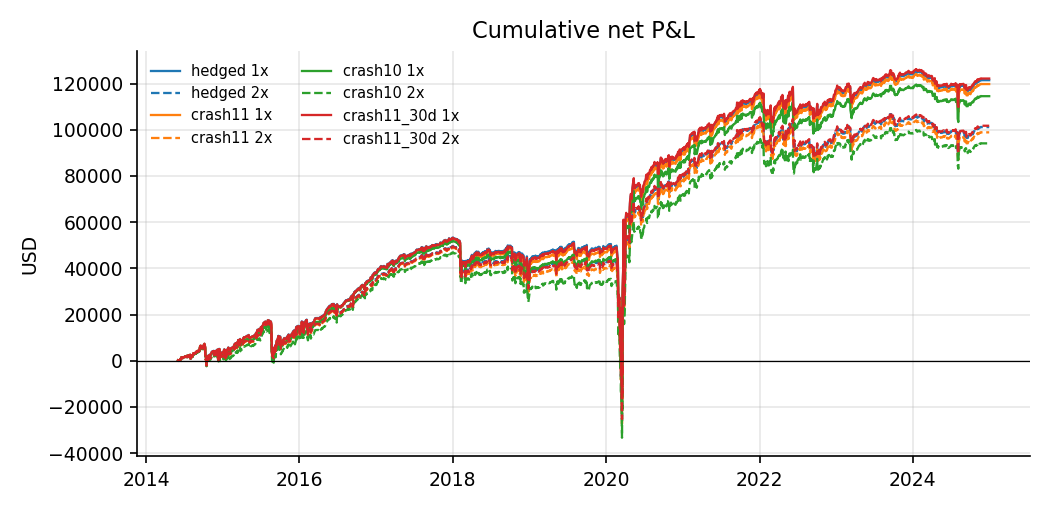
\includegraphics[width=0.92\linewidth]{figures/cum_pnl.png}\caption{Cumulative net P\&L, 1x solid and 2x dashed}\end{figure}

The four books are hard to tell apart: the crash call adds or removes a few thousand dollars over ten years on a book that makes about \$120k. Only \texttt{crash10}, which buys calls on four times as many days, sits visibly lower from 2018.

\begin{figure}[H]\centering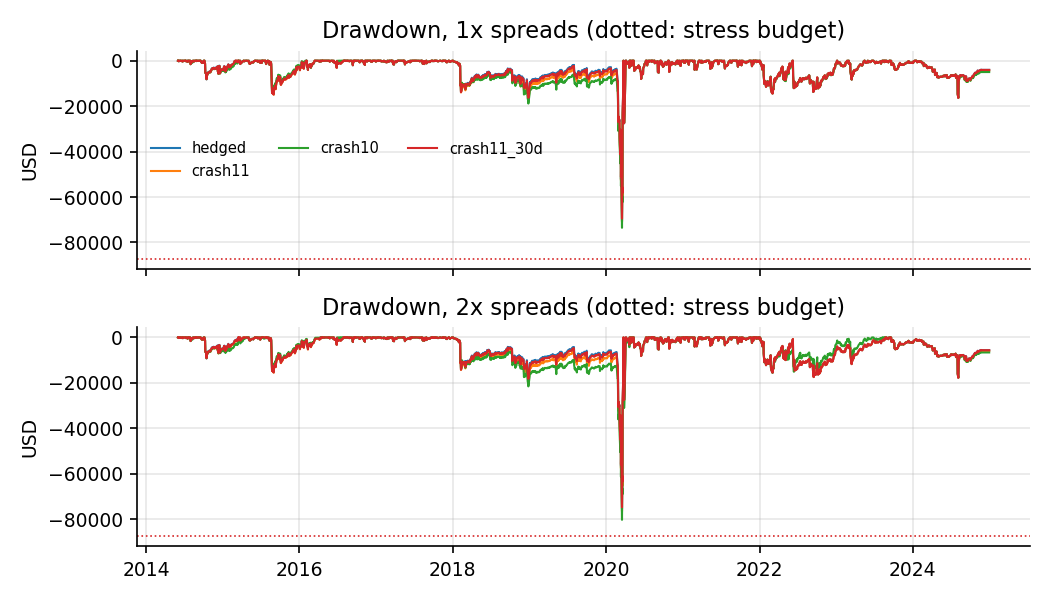
\includegraphics[width=0.92\linewidth]{figures/drawdown.png}\caption{Drawdown at 1x and 2x spreads}\end{figure}

Every book's deepest drawdown runs from 2 January 2018 to 17 March 2020, and every one stays inside the \$87,500 stress budget (dotted). \texttt{crash11} is \$636 deeper at 1x, \texttt{crash10} \$3.2k deeper, and \texttt{crash11\_\allowbreak{}30d} \$865 shallower.

\begin{figure}[H]\centering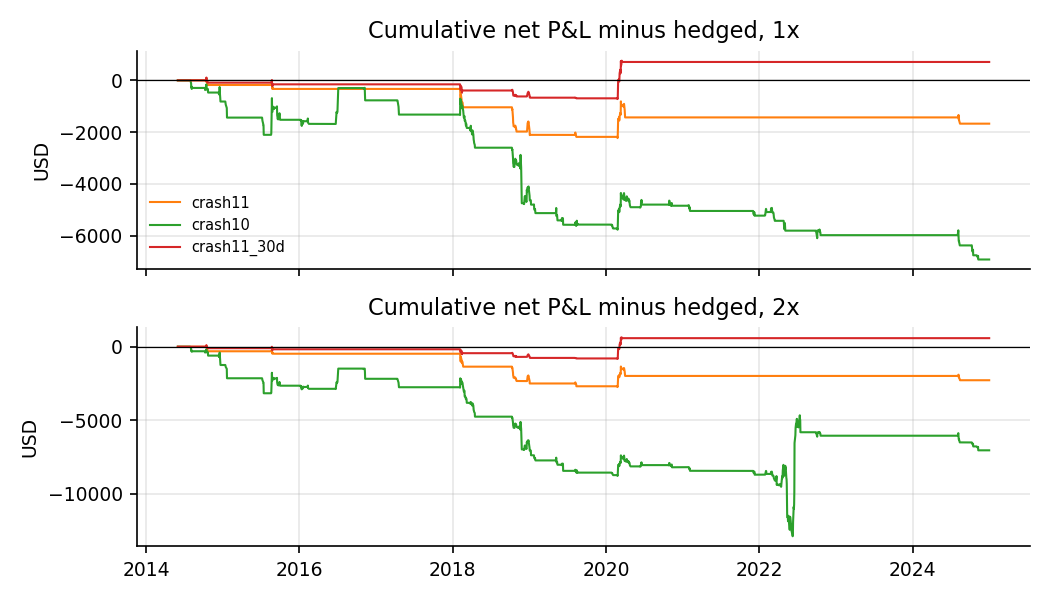
\includegraphics[width=0.92\linewidth]{figures/vs_hedged.png}\caption{Cumulative net P\&L minus hedged, at 1x and 2x}\end{figure}

This is the crash call's whole effect: each variant's cumulative P\&L minus the reference's. The put trades are the same in every book (checked below), so this difference is the calls and their share hedges. The lines step only when a call is open: down through 2018 and 2019, up in March 2020. At 2x, \texttt{crash10} jumps in mid-2022 because its put path diverges from the reference's there (see Analysis).

\begin{figure}[H]\centering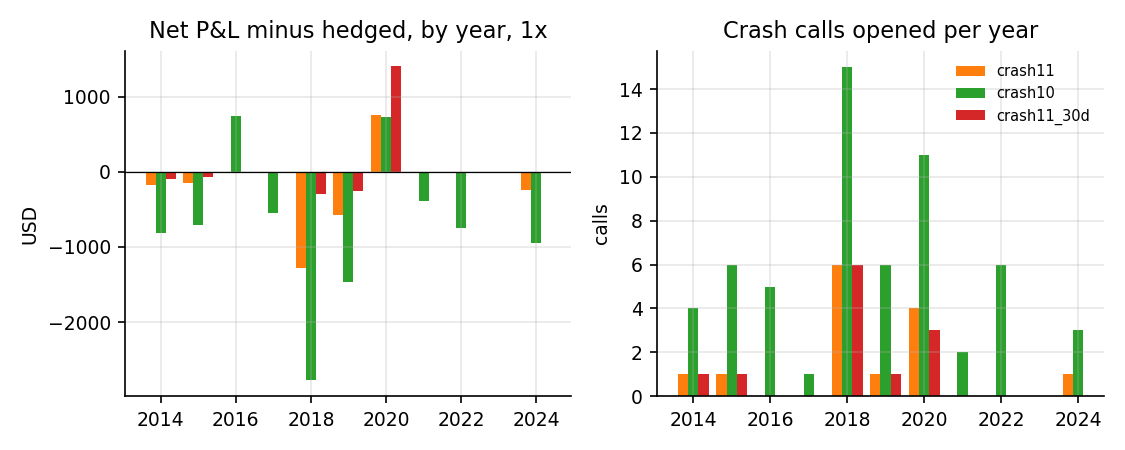
\includegraphics[width=0.92\linewidth]{figures/crash_years.png}\caption{Net P\&L minus hedged by year, and crash calls opened per year, 1x}\end{figure}

At gate 1.1 the call fires in only six of the eleven years. Most calls open in 2018 (6) and 2020 (4). It lost money in every year except 2020. At gate 1.0, \texttt{crash10} fires every year except 2023 and loses in eight of the eleven.

\begin{figure}[H]\centering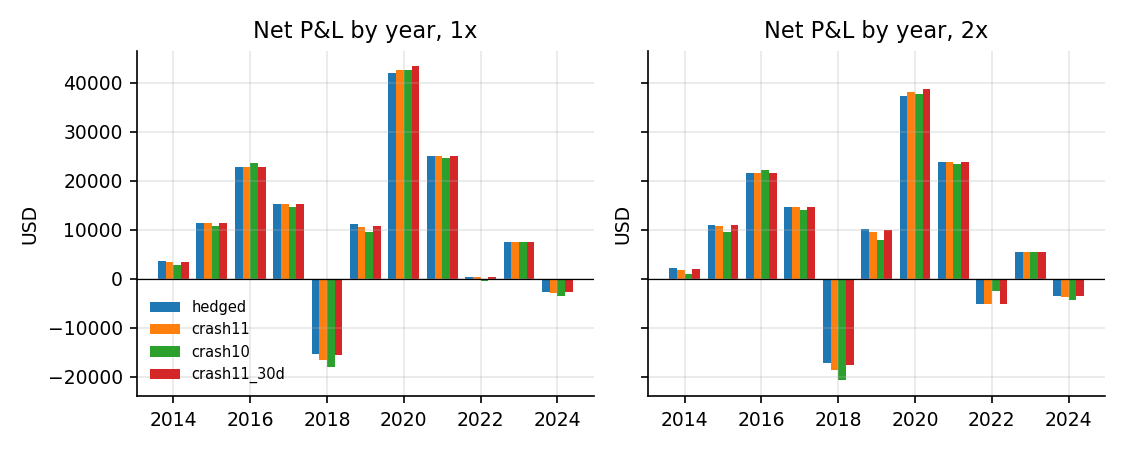
\includegraphics[width=0.92\linewidth]{figures/yearly.png}\caption{Net P\&L by year}\end{figure}

The yearly bars of the four books are close everywhere. The largest 1x gap is 2018, where \texttt{crash10} is \$2.8k below the reference at 1x.

\begin{figure}[H]\centering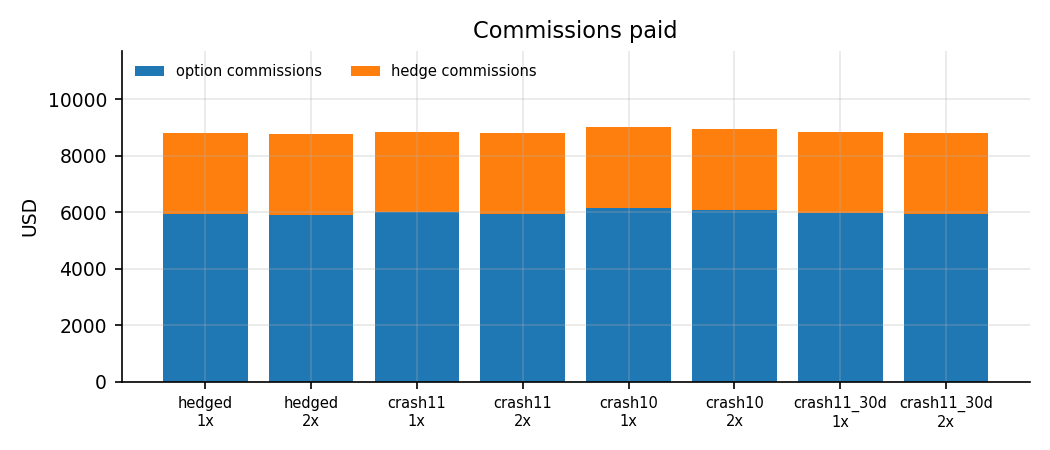
\includegraphics[width=0.92\linewidth]{figures/fees.png}\caption{Commissions paid}\end{figure}

The calls add little in commissions: \$40 at 1x for \texttt{crash11} and \$200 for \texttt{crash10}. Hedge orders and commissions barely change (2,316 orders against 2,317 at 1x), because the call's delta is added to the book's single daily hedge order.

\section{Analysis}

\textbf{The put book is the same; the difference is the calls.} At 1x, every variant opens and closes exactly the same puts as the reference, on the same days and in the same sizes. So the difference in equity is exactly the crash calls plus the shares that hedge them. At 2x, \texttt{crash10}'s puts match until March 2022. Then a profit-take fires two days later than in the reference, because the engine counts some of the call's hedge shares in the put's P\&L. Every later put is different. This path change, not the calls, causes \texttt{crash10}'s mid-2022 jump at 2x.

\textbf{The call is small.}

\begin{itemize}

\item \texttt{crash11} bought 14 calls of 1-4 contracts (2.0 on average), for \$14.6k of premium in total over ten years.

\item At the 2020 low the put book held about 100 contracts, sized to a \$87,500 stress budget. A \$1,250 call can't offset much of that.

\item Over the window the calls lost \$1,599 on their own option P\&L after commissions, and \$1,675 with their share hedges.

\end{itemize}

\textbf{The calls lost inside the drawdown window.} The reference's drawdown runs from January 2018 to 17 March 2020.

\begin{itemize}

\item In that window the calls bought after the February, October and December 2018 sell-offs and in August 2019 lost \$1.9k in 2018-2019.

\item From 19 February to 30 April 2020 they gained about \$0.75k net of hedges (their option P\&L lost \$2.8k in 2020, and the shares hedging them gained more), too little to make up the loss.

\item Net, \texttt{crash11} was \$636 behind the reference over the drawdown window, the amount by which the drawdown is deeper.

\item Net of their hedges, the calls lost money in every year with entries except 2020 (five of six).

\end{itemize}

\textbf{The sensitivities:}

\begin{itemize}

\item \textbf{A lower gate (\texttt{crash10}, 59 calls) makes it worse.} It is \ensuremath{-}\$6.9k at 1x and \ensuremath{-}\$7.0k at 2x, with a drawdown \$3.2k (1x) and \$4.8k (2x) deeper. The calls made +\$5.2k on their own option P\&L at 1x, but the shares hedging them lost \$12.1k.

\item \textbf{A 30-day call (\texttt{crash11\_\allowbreak{}30d}) meets all three checks, but only by small amounts.} It cuts the drawdown by \$865 (1x) and \$756 (2x) and adds \$709 and \$581 of P\&L. All of it is 2020 (+\$1.4k). Outside 2020 it lost \$696. It is a sensitivity, so it can't pass this card, and a gain of under \$1k decided by one episode is noise.

\end{itemize}

\textbf{What is mechanical:}

\begin{itemize}

\item The size is the pre-registered 0.5\% of capital, and the result scales with it. If fills scale, doubling the size would roughly double both the 2018-2019 losses and the March 2020 gain, so the sign would not change.

\end{itemize}

\textbf{How round trips are attributed.} The engine gives each open position a share of the book's hedge shares, so the P\&L of a single call round trip includes shares inherited from the put. One call round trip in 2015 shows a loss several times its premium on that split, while the book's total difference that year was only \ensuremath{-}\$153. This report therefore measures the call by the equity difference and by its own option P\&L, not by round-trip P\&L. The shared \texttt{report.\allowbreak{}by\_\allowbreak{}reason} chart was dropped for the same reason (see Caveats).

\section{Verdict}

\textbf{Failed} per the pre-registered bar: the maximum drawdown was worse at both spreads (\$70,998 against \$70,362 at 1x; \$76,514 against \$75,488 at 2x). ES and the P\&L allowance passed, and the floor was met (14 crash calls).

Archive this card; don't run the hold-out. At 0.5\% of capital, a crash call bought on inverted-curve days changes the put book's risk by less than \$1k either way. A meaningful hedge would have to be sized to the put book's crash loss rather than to a premium budget, and paid for over many calm inversions. That would be a different card, and the 2018-2019 losses here suggest it would cost more than it saves outside March 2020.

\section{Caveats}

\begin{itemize}

\item \textbf{Hold length.} The engine holds the call for 5 weekdays, not 5 trading days: it counts business days without the exchange calendar. Over a holiday that is 4 trading days, which happened to 3 of \texttt{crash11}'s 14 calls (February and December 2018, New Year 2019) and 5 of \texttt{crash10}'s 59. One call (August 2015) was held 6 trading days because a month-end snapshot is missing. This deviates from the card's ``5 trading days''; with 1-4 contracts it is unlikely to change the verdict, but that can't be shown without a rerun.

\item \textbf{In-sample:} the idea comes from the 2026-10-07 report and the 2026-10-22 results on 2014-2024. Before pre-registration, the gate's frequency was counted from the features file (50 days in 12 episodes at 1.1).

\item \textbf{One episode:} March 2020 is the only crash where a call pays. Every variant's sign depends on it.

\item \textbf{Hedge-share attribution:} the engine splits the book's hedge shares across open positions. Totals are right, but a single position's round-trip P\&L is not its own hedged P\&L, and at 2x it changed one put's exit in \texttt{crash10}.

\item \textbf{Report code:} \texttt{report.\allowbreak{}round\_\allowbreak{}trips} (via \texttt{metrics.\allowbreak{}pairs}) matches closes to opens by time alone. When the put and a crash call open at the same 10:15 step, it misassigns side and entry date. This card's script pairs by entry time and contract instead.

\begin{itemize}

\item The pass-bar metrics (P\&L, Sharpe, drawdown, ES) come from the equity curve and are unaffected, and so are the round-trip counts, win rate and gross.

\item The registry's \texttt{hold\_\allowbreak{}days} for this card's rows uses the time-only pairing.

\end{itemize}

\item \textbf{Spread model:} fitted on about two weeks of calm 2026 live quotes. Short-dated at-the-money calls in a spike may cost more than modelled; the 2x run is the stress test.

\item \textbf{Data gaps:} R2 has no month-end weekdays, so about 3.3\% of scheduled times are skipped.

\item \textbf{Gate timing:} the gate reads the prior close, like every desk gate. A same-day trigger could enter a day earlier in a crash.

\end{itemize}

\section{Trials}

6 trials for this experiment (3 variants \ensuremath{\times} 1x and 2x, one run of \texttt{experiment.\allowbreak{}py}). No new baseline was needed, and the reference was reused, not rerun. The registry holds 134 trials at the time of writing.

All six rows are tagged \texttt{3568520-\allowbreak{}dirty}: other cards of the same batch had uncommitted files in the shared working tree. The engine, the configs and this card's files were unchanged since pre-registration.

After the run, the charts were changed in the script only and rebuilt with \texttt{-\allowbreak{}-\allowbreak{}report-\allowbreak{}only}, which adds no trials:

\begin{itemize}

\item the shared by-reason chart was replaced by cumulative P\&L minus \texttt{hedged};

\item the crash-call P\&L panel now uses the equity difference.

\end{itemize}

The pass bar was not changed.

\end{document}
